% format de la feuille
% taille police globale (pas les titres)
% recto (oneside) ou recto-verso (twoside)
% fleqn pour numéroter les équations à droite
% classe : article, book, report
\documentclass[a4paper,fleqn,12pt]{report}

% ---------------------------------------------------------------------------------------------------------
% LANGUES ET POLICE
\usepackage[francais]{babel} % langue principale : français
\usepackage[utf8]{inputenc} % encodage 
\usepackage[T1]{fontenc} % accents
\usepackage{lmodern} % police vectorielle
\usepackage{ulem} % souligner
\usepackage[usenames,dvipsnames,svgnames,table]{xcolor} % pour écrire en couleur 

% ---------------------------------------------------------------------------------------------------------
% CARACTERES SPECIAUX + MATH
\usepackage{csquotes} % beaux guillemets \enquote{texte}
\usepackage{amssymb} % symboles mathématiques
\usepackage{listings} % inclure du joli code
\usepackage{listingsutf8}
\usepackage{amsmath} % formules mathématiques, flèches etc
\usepackage{amsfonts} % fraktur etc. 
\newcolumntype{M}[1]{>{\raggedright}m{#1}}
\lstset{
  language=Java,
  basicstyle=\ttfamily,
  columns=fullflexible,
  frame=single,
  breaklines=true,
  postbreak=\mbox{\space},
  numbers=left,
  numberstyle=\tiny,
  showspaces=false,
  showtabs=false,
  showstringspaces=false,
  breakatwhitespace=true,
  commentstyle=\color{MidnightBlue},
  keywordstyle=\color{blue},
  stringstyle=\color{ForestGreen},
  moredelim=[il][\textcolor{gray}]{\$\$},
  moredelim=[is][\textcolor{gray}]{\%\%}{\%\%},
  literate=%
         {é}{{\'e}}1
         {è}{{\`e}}1
         {ú}{{\'u}}1   
         {ù}{{\`u}}1
         {Á}{{\'A}}1
         {É}{{\'E}}1
         {ê}{{\^e}}1
         {Ê}{{\^E}}1
         {œ}{{\oe}}1
         {â}{{\^a}}1
         {à}{{\`a}}1
}
\lstdefinelanguage{json}{
    basicstyle=\normalfont\ttfamily,
    numbers=left,
    numberstyle=\scriptsize,
    stepnumber=1,
    numbersep=8pt,
    showstringspaces=false,
    breaklines=true,
    frame=lines,
    backgroundcolor=\color{white},
    literate=
     *{0}{{{\color{MidnightBlue}0}}}{1}
      {1}{{{\color{MidnightBlue}1}}}{1}
      {2}{{{\color{MidnightBlue}2}}}{1}
      {3}{{{\color{MidnightBlue}3}}}{1}
      {4}{{{\color{MidnightBlue}4}}}{1}
      {5}{{{\color{MidnightBlue}5}}}{1}
      {6}{{{\color{MidnightBlue}6}}}{1}
      {7}{{{\color{MidnightBlue}7}}}{1}
      {8}{{{\color{MidnightBlue}8}}}{1}
      {9}{{{\color{MidnightBlue}9}}}{1}
      {:}{{{\color{black}{:}}}}{1}
      {,}{{{\color{black}{,}}}}{1}
      {\{}{{{\color{ForestGreen}{\{}}}}{1}
      {\}}{{{\color{ForestGreen}{\}}}}}{1}
      {[}{{{\color{ForestGreen}{[}}}}{1}
      {]}{{{\color{ForestGreen}{]}}}}{1},
      literate=%
         {é}{{\'e}}1
         {è}{{\`e}}1
         {ú}{{\'u}}1
         {ù}{{\`u}}1
         {Á}{{\'A}}1
         {É}{{\'E}}1
         {ê}{{\^e}}1
         {Ê}{{\^E}}1
         {œ}{{\oe}}1
         {à}{{\`a}}1
}
% ---------------------------------------------------------------------------------------------------------
% LISTES
\usepackage{enumitem} % customiser les listes
%\frenchbsetup{StandardLists=true} % éviter les conflits avec enumitem
\setlist[itemize]{noitemsep, topsep=0pt}
\setlist[enumerate]{noitemsep, topsep=0pt}
\setlist[description]{noitemsep, topsep=0pt}
% ---------------------------------------------------------------------------------------------------------
% TABLEAUX ET FIGURES
\usepackage[sc,footnotesize]{caption} % légendes des tableaux et figures
\usepackage{subfig} % plusieurs figures côte à côte (subfloat)
\usepackage{longtable} % autoriser que les longs tableaux débordent sur plusieurs pages
\usepackage{multicol} % fusionner les colonnes dans un tableau
\usepackage{multirow} % fusionner les lignes dans un tableau
\usepackage{caption} % pour les légendes
\usepackage{slashbox} % pour les Tableaux comparatifs
\usepackage{graphicx} % insérer image
\usepackage{rotating}
\usepackage{epstopdf}
\usepackage{wrapfig}

\usepackage{fancybox}
\graphicspath{{figures/}} % dossier dans lequel sont les images
%\usepackage{tikz} 	% outil de modélisation de formes

% ---------------------------------------------------------------------------------------------------------
% MISE EN PAGE 
\usepackage{lscape}
\usepackage{setspace}
\usepackage{verbatim}
\usepackage{url}
\bibliographystyle{plain}

\raggedbottom

% - Marges
\usepackage[top=2cm, bottom=2cm, left=2cm, right=2cm ]{geometry} % marges

% - Page style
\pagestyle{headings}

\DeclareUnicodeCharacter{00A0}{ }
% - Alinéas et espacements entre paragraphes
\usepackage{parskip}
\parskip = 10pt % espace
\parindent = 0pt % alinéa

% - Style des sections
\usepackage{titlesec}
\titleformat*{\section}{\Large\scshape}
\titleformat*{\subsection}{\large\scshape}
\titleformat*{\subsubsection}{\scshape}

\pagestyle{plain}
%---------------------------------------------------------------------------------------------------------
\selectlanguage{francais}
\author{Gilles Bodart}
\date{\today}
\title{Archipelago}
\begin{document}
\thispagestyle{empty}

\begin{center}
\textsc{Universit\'e de Namur}\\
Facult\'e d'informatique\\
Ann\'ee acad\'emique 2017--2018
\end{center}
\vspace{1.3cm}
\hspace{1.4cm}
\begin{center}
\fbox{
\begin{minipage}[c][5.4cm]{11cm}
\large
\begin{spacing}{1.2}
\begin{center}
\textbf{Archipelago : Un framework de persistance pour bases de données orientées graphe.}
\\
\vspace{0.5cm}
Gilles Bodart
\end{center}
\end{spacing}
\end{minipage}
}
\end{center}


\vspace{0.5cm}
\begin{figure}[!h]
\centering
\includegraphics[width=.4\textwidth]{figures/unamur.pdf}
\end{figure}

\normalsize


\vspace{0.5cm}
\begin{table}[!h]
\centering
  \begin{tabular}{ r l }
    Promoteur~: &  \rule{4cm}{0.1mm} {\small (Signature pour approbation du d\'ep\^ot - REE art. 40)}\\
    ~\underline& CLEVE Anthony \\\\
    Co-promoteur~: & LAMBIOTTE Renaud  \\
  \end{tabular}
\end{table}

\vspace{0.5cm}
\begin{center}
M\'emoire pr\'esent\'e en vue de l'obtention du grade de\\
Master en Sciences Informatiques.
\end{center}

\section*{Résumé}

Ce mémoire va se concentrer sur les implémentations de la théorie des graphes dans l'univers des bases de données, et développer un framework Java présentant les qualités suivantes, l'abstraction, la simplification et la configurabilité. 

Archipelago est un framework dont le but est d'abstraire l'utilisation d'une base de données orientée graphe. Cet outil dans son  état actuel, possède trois méthodes fonctionnelles, à savoir une méthode permettant de persister l'information, une autre permettant de lier deux noeuds à l'aide d'une relation, et une dernière permettant de récupérer les différents objets dans la base de données. Elle peut effectuer ces trois opérations sur \texttt{Néo4J} et sur \texttt{OrientDB}.

Ce travail présente les points forts et les points faibles de l'implémentation de ce framework ainsi que des pistes d'amélioration pour une version ultérieure.

\quad \quad \underline{mots-clés :} Framework, Base de données, Java, Graphes, Neo4J, OrienDB, Archipelago
\section*{Abstract}

In the scope of this master thesis, a new Java framework was developed to apply the graph theory to databases. This framework presents interesting qualities, such as abstraction, simplification and configurability. 

Archipelago framework abstracts graph-oriented databases. Currently, three methods are available: a first method that persists information, a second method that links nodes together with the help of a relation with or without properties and a third method that gives the ability to query databases and to retrieve persisted objects states. The framework can be used with both \texttt{Néo4J} and \texttt{OrientDB}.

This master thesis presents the framework implementation, its applications and its strengths and weaknesses.

\quad \quad \underline{keywords :} Framework, databeses, Java, Graphs, Neo4J, OrienDB, Archipelago

\chapter*{Avant-propos}

Nous tenons à remercier tout particulièrement mes promoteurs, Messieurs A. CLEVE et R. LAMBIOTTE pour nous avoir autorisé à réaliser cette recherche et conjointement, à nous avoir soutenu dans le développement de celle-ci. Nous les remercions aussi pour le temps consacré à la supervision de ce mémoire. 

Nous remercions également les entreprises dans lesquelles nous avons travaillé, de nous avoir laissé l'opportunité de poursuivre le cursus universitaire.

Et enfin, nous tenons tout autant à remercier ma belle-mère C. NIGOT pour avoir pris du temps à nous relire, et singulièrement ma compagne M. VAN CUTSEM qui m'a soutenu au quotidien pendant ces deux années, y compris pour sa patience actuelle durant sa grossesse en cours.


\tableofcontents
\newpage
\chapter*{Glossaire}
\begin{center}
\begin{tabular}[c]{ l p{14cm} }
 SQL  & Structured Query Language \\ \hline
 NoSQL  & Not only SQL \\ \hline
 SGBD  & Système de gestion de base de données \\ \hline
 SGBDR  & Système de gestion de base de données relationnelles \\ \hline
 BDOG  & Base de donnée orientée graphe \\ \hline
 JSON  & JavaScript Object Notation \\ \hline
 Vertex  & Sommet \\ \hline
 Edge  & bord \\ \hline
 Cluster  & littéralement grappe, cela représente en informatique un groupe d'éléments \\ \hline
 API  & Application Programming Interface  \\ \hline
 REST  & Representational state transfer, style d'architecture pour les systèmes hypermédia distribués \\ \hline
\end{tabular}
\end{center}

\chapter*{Introduction}

De nos jours, les unités de stockage sont de plus en plus accessibles au grand public, les différentes entreprises impliquées dans le développement des systèmes de gestion de base de données l'ont bien compris. Depuis plusieurs années, l'hégémonie des bases de données relationnelles se fait de moins en moins écrasante, les solutions alternatives du NoSql séduisent jour après jour de grandes entreprises. 

La grande force des SGBDR provient des fondements théoriques mis en place en 1970 par Edgar Frank Codd. IBM définit le langage "Structured Query Language" (SQL) pour utiliser ce système. Cette normalisation de la représentation de l'information génère un sentiment de sûreté pour les architectes de logiciels.

A contrario, le mouvement NoSql pour "Not Only SQL" ne se base pas sur un fondement théorique commun. Que ce soient la théorie des graphes, les systèmes de hash key/value avec partitions, ... chaque système choisit ce sur quoi il va se baser. 

Mais s'il existait une sorte de contrat liant les SGBD NoSql entre eux afin d'assurer une cohérence d'utilisation, ce mémoire va se concentrer sur les implémentations de la théorie des graphes, en essayant de mettre en place un système de comparaison. Nous allons tenter de spécifier certains objectifs communs et développer un framework Java permettant d'utiliser de manière agnostique l'une ou l'autre base de données.

En outre, nous aimerions produire un framework qui présente les qualités suivantes :
\begin{itemize}
\item[•] L'abstraction

\quad L'utilisateur pourra employer ce framework sans même connaitre l'existence de librairies spécifiques.
\item[•] La simplification

\quad Les différentes méthodes seront explicites et faciles à intégrer dans une application existante.
\item[•] La configurabilité 

\quad Le framework réagira en fonction d'un fichier de configuration clair et simple.
\end{itemize}
 
\part{État de l'art}

\chapter{L'évolution du NoSql}
\label{NoSqlEvol}


1.

Un SGBD est par définition un ensemble de procédés permettant d'organiser et de stocker des informations (potentiellement de gros volumes). Si stocker et retrouver l'information est un des plus grand challenge d'un SGBD, une communauté de développeur pense que ces systèmes devraient pouvoir offrir d'autres fonctionnalités. 

A partir des années 1980, le modèle relationnel supplante les autres formes de structures de données.

Les évolutions logicielles suivant naturellement les évolutions matérielles, la généralisation des interconnexions des réseaux, l'augmentation de la bande passante, la diminution du coût des machines, la miniaturisation des espaces de stockage, ... de nouvelles opportunités sont apparues au XXI\up{e} siècle.

Les entreprises comme Google, Amazon, Facebook, Twitter, ... sont tour à tour arrivées aux limites du modèle relationnel. Que ce soit à cause de volumes astronomiques (plus de 100 pétaoctets) ou du nombre de requêtes par seconde, il fallut développer une nouvelle façon de gérer les données.

Le NoSql découle de ce genre de problèmes, ces modèles arrivent avec des approches optimisées pour des secteurs spécifiques. \\
Comme ces modèles représentent ce qui n'est pas relationnel, par souci de classification, nous allons distinguer 4 usages principaux :

\begin{itemize}
\item Performances : L'objectif du SGBD sera d'augmenter au maximum les performances de la manipulation des données. 
\item Structures simples : Pour s’affranchir de la rigidité du modèle relationnel, la structure sera généralement simplifiée, en utilisant une représentation plus souple comme le JSON par exemple.
\item Structures spécifiques : Certains moteurs NoSql sont liés à des besoins spécifiques. La structure de représentation de données sera dès lors focalisée sur un cas d'utilisation.
\item Volumétries : Un des principaux aspects importants des SGBD NoSql est leur capacité de gérer la montée en charge de données. La distribution des traitements au travers de plusieurs clusters est un facteur essentiel dans la plupart des applications BigData.
\end{itemize} 

Nous allons aussi distinguer 4 grandes familles de représentation de schéma de données :

\begin{itemize}
\item Document : L'utilisation de formats spécifiques tels que le très répandu "JSON" permet de stocker les données sur base de fichier.
\item Clé / Valeur : Le système le plus simple, il manipule des paires de clé/valeur, ou accède à un élément en fonction d'une table de hachage.
\item Colonne : Inspiré de Google BigTable, la structure ressemble à la table relationnelle. On peut la comparer à une table de hachage qui va référencer une ou plusieurs colonnes.
\item Graphe : La famille Graphe se distingue du fait que les entités ne sont pas considérées comme des entités indépendantes, mais que la relation entre ces objets est tout aussi importante que le contenu.
\end{itemize} 

Les implémentations de bases de données de types graphe sont de plus en plus nombreuses, les relations entre les éléments permettent de parcourir le graphe de manière très performante le rendant de plus en plus intéressant pour les entreprises possédant des millions de données. L'utilisation de ce genre de SGBD est dès lors tout à fait recommandée pour des entreprises intéressées entre les relations de ces données, telles que des profils sociaux, des liens de cause à effet, des liens géographiques et bien d’autres encore.\cite{infoqSite}\cite{NoSqlDef}\cite{bruchez2016bases}

\section{Questionnement}

\subsection*{Pourquoi utiliser une BDOG plutôt qu'une BD relationnelle comme Oracle ou MySql ?}

L’utilisation des SGBD relationnelles pour tout type de problème est révolue. L’apparition de SGBD NoSQL spécifiques, permet dès à présent une approche plus personnalisée. En effet, comme tout système, le relationnel a ses limites. L’approche actuelle des entreprises est plus orientée "Big Data" ; les entreprises veulent tout stocker afin d’avoir le plus d’informations possible. Or comme le relationnel cadenasse les données dans une table préalablement définie, on se doit de tronquer l’information ou de mettre à jour le schéma de définition des tables. Dans une BDOG telle que Neo4J, nous pouvons ajouter toutes les informations que nous voulons sans condition préalable. Cette approche permet davantage un contrôle de l’intégrité des données aux applications.

Si l’objectif de l’applicatif est de représenter un système récursif comme une arborescence de fichier, de la généalogie, ... le modèle relationnel se basera sur une table faisant référence à elle-même, l’utilisateur devra donc réaliser une jointure par profondeur. Si l’arborescence descend jusqu’à 15 niveaux, cela peut devenir problématique. L’approche BDOG permet de parcourir une arborescence sans pour autant charger l’ensemble des nœuds ayant le même label. Dès lors, plus besoin de projection "d’ensemble" pour pouvoir continuer le chemin.

En relationnel, il existe de nombreux moyens d’historiser les données, cependant, lorsque le schéma comprend des relations cycliques, cette opération devient plus complexe. L’utilisation d’un BDOG rend la démarche plus simple, il suffit de créer un nouveau nœud avec les anciennes données, lier ce nœud avec une relation historique en y spécifiant la date de mise à jour, et ensuite de changer les valeurs du nœud référencé par le cycle. Ce procédé peut être mis au point dans n’importe quelle représentation et ne nécessite aucune refonte globale du modèle de données.\cite{NoSQLVsSGBDR}\label{noSqlVSRel}

\subsection*{On parle de base de données orientée graphe mais quelle est la différence entre une relation entre deux nœuds et une relation entre deux tables ?}
Les relations entre deux tables se font à l’aide de clé étrangère définie lors de la création du schéma de données. Elles apportent de l’information supplémentaire en permettant de réaliser des jointures entre plusieurs tables.

La relation dans les BDOG est une information à part entière, elle peut posséder autant de données que le nœud lui-même, la force de ce genre de système est de pouvoir lier deux nœuds distincts par n’importe quelle relation et ce, à tout moment.

\chapter{Backgroud technique}
\section{Neo4J}

\subsection{Description}

Créé par Neo Technologie, une société américaine et suédoise, elle est actuellement la base de données orientée graphe, la plus utilisée dans le monde\cite{DBEnginesSite}. Développé en java sous licence GPL V3, AGPL ou licence commerciale, Neo4J représente les données sous forme de "Nœuds" et de "Relations". Chacun de ces éléments peuvent contenir une ou plusieurs propriétés. Les propriétés sont des couples clés/valeurs de type simple, comme des chaines de caractères ou des valeurs numériques, des coordonnées spatiales, ... \cite{Neo4JSite}

Une des particularités de Neo4J est l’absence de structure définie, un nœud peut être labellisé afin de permettre de travailler sur un ensemble d’éléments, mais il n’y aura aucune contrainte sur les propriétés du nœud. Cette particularité rend ce SGBD bien adapté pour les modèles évoluant fréquemment.


\subsection{Langage de requête}

Le langage propre à Neo4J se nomme "Cypher"\label{Cypher}, il a pour but de réaliser plus simplement que SQL les opérations de parcours ou d'analyse de proximité.

\begin{lstlisting}[language=java, frame=single]
CREATE (mamours:Person {name:"Mamours"})
CREATE (mamyco:Person {name:"Mamyco"})
CREATE (gilles:Person {name:"Gilles"})
CREATE (marie:Person {name:"Marie"})
CREATE (bebe:Person {name:"Enfant"})
CREATE (mamours)-[:PARENT_OF]->(gilles)
CREATE (mamyco)-[:PARENT_OF]->(marie)
CREATE (marie)-[:PARENT_OF]->(bebe)
CREATE (gilles)-[:PARENT_OF]->(bebe)
\end{lstlisting}

Ces requêtes vont créer 5 nœuds et 4 relations PARENT\_OF, nous pouvons aisément comprendre que "Mamyco" est parente de "Marie"

\begin{lstlisting}[language=java, frame=single]
MATCH (p:Person)-[:PARENT_OF]->(c:Person) 
RETURN DISTINCT (p)
	
\end{lstlisting}

Cette query va retourner tous les nœuds distincts qui ont une relation :PARENT\_OF avec un autre nœud.

\begin{lstlisting}[language=java, frame=single]
MATCH (gp:Person)-[:PARENT_OF*2]->(c:Person) 
RETURN DISTINCT (gp)
	
\end{lstlisting}

Celle-ci quant à elle va retourner toutes les personnes qui sont "parent de parent" et donc grands-parents. 

Ces deux exemples peuvent montrer la force de l’utilisation d’un SGBD de type graphe pour représenter un ensemble hiérarchique de données par rapport aux SGBD relationnels qui nécessiteraient une double jointure sur la Table "Person".

\subsection{Communication}

Neo4J peut être utilisé sous plusieurs formes.

La première option est une solution embarquée, ce choix peut être très intéressant en alternatif au très célèbre SQLite relationnel.

La deuxième, pour toute application distribuée, est une solution autonome pouvant tourner comme un service sur tout type de plateforme. Le protocole "Bolt", développé par "Néo Technologie" est grandement conseillé pour communiquer avec ces serveurs distants.

Son utilisation est simple grâce à l’utilisation de la librairie native à Néo4J pour java (neo4j-java-drive) ou avec l’utilisation de l’API Rest déployée en même temps que le SGBD.

\section{OrientDB}

\subsection{Description}

OrientDB est un SGBD initialement développé en C++ (Orient ODBMS), repris ensuite en 2010 en Java par Luca Garulli dans une version multi-modèle sous licence Apache 2.0, GPL et AGPL. Actuellement 3ème mondial (selon db-engines.com) il offre de nombreuses fonctionnalités intéressantes.\cite{OrientDBSite}

OrientDB est une base de données associant Document et Graphe. Elle combine la rapidité et la flexibilité du type document ainsi que les fonctionnalités de relations des bases de données graphe.

Ce SGBD est composé de trois grands éléments 

\begin{itemize}
\item Document \& Vertex : Source de contenu, ces éléments peuvent être considérés comme des containers de données. On peut le comparer avec la ligne d'une base de données relationnelles.
\item Links \& Edge : Une arête orientée reliant deux éléments non nécessairement distincts.
\item Property : Typée ou embarquée dans un document JSON, ceci va représenter le contenu de l'information. Ces propriétés sont bien entendu primordiales pour ordonner, rechercher, ...
\end{itemize}

Chaque Document ou Vertex appartient à une "Class", celle-ci peut être strictement définie ou plus laxiste. Comme dans la programmation orientée objet, OrientDB offre le principe de polymorphisme avec un système d'héritage entre les classes. 

OrientDB vient dans sa version community avec un système de clustering permettant à l’utilisateur de gérer correctement les montées en charge. Chaque document est identifié avec une partie désignant le cluster dans lequel l’information est stockée et une autre partie désignant sa position dans ce dernier (exemple @rid: 10:12). Chaque classe peut être associée à un ou plusieurs clusters, permettant d’optimiser les accès dans des ensembles plus petits.


\subsection{Langage de requête}

OrientDB utilise une sorte de SQL avancée pour interpréter les requêtes. On peut de plus utiliser le langage Gremlin.

Voici quelques exemples d'utilisation du SQL avancé dans OrientDB.

\begin{lstlisting}[language=SQL]
CREATE CLASS Person EXTENDS V
CREATE CLASS Company EXTENDS V
CREATE CLASS WorkAt EXTENDS E
CREATE PROPERTY Person.firstname string
CREATE PROPERTY Person.lastname string
CREATE PROPERTY Company.name string
INSERT INTO Person(firstname, lastname) VALUES ("Gilles","Bodart"),("Marie","Van Cutsem")
	ou
INSERT INTO Company set name = "ACME"

\end{lstlisting}

Cet ensemble de requêtes ressemblant au langage SQL permet de créer deux vertex, Person et Company, un Edge WorkAt et leur associe certaines propriétés. Les deux types d’insert différents permettent comme en SQL d’ajouter un nœud.

\begin{lstlisting}[language=SQL]
SELECT FROM V
\end{lstlisting}
\begin{center}
	\begin{tabular}{|c|c|c|c|c|c|}
   		\hline
  		\multicolumn{3}{|c|}{Metadata} & \multicolumn{3}{c|}{Properties} \\
   		\hline
   		@rid & @version & @class & firstname & lastname & name \\
   		\hline
   		10:0 & 1 & Person & Marie & Van Cutsem &  \\
   		10:1 & 1 & Person & Gilles & Bodart &  \\
   		11:0 & 1 & Company &  &  & ACME \\
   		\hline
	\end{tabular}
\end{center}

Nous pouvons observer qu'OrientDB se charge de qualifier les documents de plusieurs métadata en leur octroyant par exemple un identifiant unique (\no cluster:position), un numéro de version pour permettre une gestion de transaction "full optimistic"\footnote{On laisse l'utilisateur continuer sa transaction et le refus se fera lors du "commit" s'il y a eu une modification concurrente du même document} et le \@class représente la structure du document.

\begin{lstlisting}[language=SQL]
CREATE Edge WorkAt from 10:1 to 11:0
\end{lstlisting}

Cette petite requête va lier le document ayant l'id 10:1 au document dont l'id est 11:0 par une relation WorkAt. Nous pouvons traduire en français que Marie Van Cutsem travaille chez ACME.\cite{OrientDBGettingStarted}


\subsection{Communication}

OrientDB embarque une API Rest complète\cite{fielding2000architectural}, toute action pouvant être faite sur les interfaces web et consoles, peut être reproduite au travers de cette API.

Outre la communication via le protocol \texttt{http}, nous pouvons aussi accéder à la base de données via une des trois librairies java développée par OrientDB.


\chapter{Solutions existantes}


\section{Les librairies} 

\textcolor{blue}{TODO livre}

\subsection{Hibernate}

Hibernate, soutenu et développé par JBoss, a mis au point un système de relation entre le code Java et le SGBD Néo4J, en réutilisant les mêmes annotations de relations que celles employées pour les bases de données relationnelles, à savoir :

\begin{itemize}
\item @OneToOne : Relation 1-1
\item @ManyToOne : Relation n-1
\item @OneToMany : Relation 1-n
\item @ManyToMany : Relation n-n
\end{itemize}

Bien qu'à l'heure actuelle, aucune intégration avec OrientDB, un ticket est ouvert (OGM-855) depuis 2 ans auprès d'Hibernate.

\subsection{Spring Data}

Spring data à nouveau possède un module de communication avec le SGBD Néo4J, il intègre au célèbre Framework Spring, les fonctionnalités de Néo4J-OGM\footnote{Object Graph Mapper}, permettant de qualifier une classe avec certaines annotations facilitant la sérialisation et la dé sérialisation vers la représentation graphique.

Exemple : 

\begin{lstlisting}
@NodeEntity(label="Film")
public class Movie {

   @GraphId Long id;

   @Property(name="title")
   private String name;
}

@NodeEntity
public class Actor extends DomainObject {

   @GraphId
   private Long id;

   @Property(name="name")
   private String fullName;

   @Relationship(type="ACTED_IN", direction=Relationship.OUTGOING)
   private List<Role> filmography;

}

@RelationshipEntity(type="ACTED_IN")
public class Role {
    @GraphId   
    private Long relationshipId;
    @Property  
    private String title;
    @StartNode 
    private Actor actor;
    @EndNode   
    private Movie movie;
}
\end{lstlisting}

\subsection{Librairie Neo4J}

Une librairie java développée par NeoTechnologie existe, elle permet de travailler aisément avec une base de données Neo4J embarquée ou à distance. Elle est en constante évolution et se trouve sur une plateforme open source. 

Exemple de communication avec la librairie Neo4J le protocol "Bolt":

\begin{lstlisting}[language=java]
Driver driver = GraphDatabase.driver("bolt://localhost:7687", AuthTokens.basic("matrix", "neo"));
Session session = driver.session();
session.run("CREATE (a:Person {firstName:{name},lastName:{lastName}})", parameters("firstName","Gilles","lastName","Bodart"));
session.close();
driver.close();

\end{lstlisting}

Bien que cette libraire soit efficace, elle ne peut être utilisée avec un autre SGBD. 

\subsection{Librairie OrientDB}

La librairie OrientDB pour java est composée de trois éléments:

\begin{itemize}
\item \texttt{graph API}
\item \texttt{document API}
\item \texttt{object API}
\end{itemize}

La \texttt{graph API} d’OrientDB couvre 80\% des uses cases classiques d’un utilisateur, elle supporte tous les modèles de représentations comme un unique multi-modèle de données. Elle travaille sur des "Vertex" et des "Edges", respectivement nœuds et relations, et est compatible avec le standard TinkerPop

La \texttt{document API} permet de couvrir les 20\% restants, il est plus simple d’utilisation mais offre une utilisation plus atomique, les relations ne peuvent être par exemple qu’unidirectionnelles tandis que la bidirectionnalité est offerte dans l’API précédent. Un document API est un élément unique pour gérer les relations entre les différents nœuds de notre modèle, il faudra gérer manuellement chaque connexion.

La dernière librairie se focalise sur les objets java, elle n'a plus été améliorée depuis la version 1.5 d'OrientDB\footnote{À l'heure de l'écriture de ce mémoire, nous sommes à la version 2.2 et la version 3 a bientôt terminé sa phase de "bêta test"}

\section{Les frameworks}

\subsection{Apache TinkerPop}

Apache TinkerPop est un Framework open source d’utilisation de graphe, il regroupe un grand ensemble de fonctionnalités et d’algorithmes. Son écosystème est de plus en plus agrémenté de librairies externes développées par de tierces personnes.

Il se considère lui-même comme étant d’utilisation complexe pour les nouveaux développeurs car il nécessite l’utilisation d’un environnement qui lui est propre, la "Gremlin-console".

Les développeurs de ce framework ont mis au point un langage de travail sur les graphes appelé "Gremlin". Le langage dont nous avons parlé en section \ref{Cypher} s’est grandement inspiré de ce dernier.\cite{tinkerPopSite}

Exemple d’utilisation

\begin{lstlisting}
gremlin> g.V() /* récupère tous les nœuds du graphe */
==>v[1]
==>v[2]
==>v[3]
==>v[4]
==>v[5]
==>v[6]
gremlin> g.V(1) /* récupère le nœud d'Id 1 du graphe*/
==>v[1]
gremlin> g.V(1).values('name') /* récupère le nœud d'Id 1 du graphe et renvoie sa propriété 'name' */
==>marko
gremlin> g.V(1).outE('knows') /* récupère les relations 'knows' partant du noeud d'Id 1 */
==>e[7][1-knows->2]
==>e[8][1-knows->4]
gremlin> g.V(1).outE('knows').inV().values('name') /* retourne le nom des personnes que le nœud 1 connait */
==>vadas
==>josh
gremlin> g.V(1).out('knows').values('name') /* même résultat */
==>vadas
==>josh
gremlin> g.V(1).out('knows').has('age', gt(30)).values('name') /* retourne le nom des personnes âgées de plus de 30 ans que le nœud 1 connait */
==>josh
\end{lstlisting}

Comme expliqué plus haut, le langage doit être exécuté dans une invite de commande ou dans un serveur Gremlin, nous sommes dès lors contraints d’installer et de configurer ce dernier pour pointer vers l’un ou l’autre SGBD.



\part{Contribution}
\chapter{Applications possibles des BDOG}

\section{L'exemple parfait}

Pour la suite de ce mémoire, il est primordial d'avoir un exemple concret de modèle habituellement persisté avec un modèle relationnel mais qui pourrait néanmoins être transposable dans une BDOG.

\subsection*{L'école}

Imaginons la représentation d'une école composée d'élèves, de professeurs, de classes, de salles techniques, de travailleurs, ... dont   le diagramme de classes se trouve en Annexe (\ref{fig:SchoolDiagram}).

Les liens entre les différents objets peuvent être très nombreux, nous pouvons imaginer que les étudiants sont amis, membres de famille, ennemis, amoureux, ... il en est de même pour les professeurs, ils peuvent avoir les mêmes relations que les étudiants mais en outre ils vont être assignés à des cours, à des classes, ... toutes ces liaisons peuvent être fortement compliquées à représenter sur une base de donnée relationnelles. L’utilisation d’une BDOG dans ce cas, semble tout à fait adéquate. Durant la suite de ce mémoire, nous utiliserons donc ce modèle.

\section{Critères de comparaison}

Dans un premier temps, il est primordial de mettre en place une liste de critères permettant de faciliter le choix de la BDOG.

\section{Comparaison des plus grandes BDOG} 
\begin{center}

\begin{tabular}[c]{|l|M{5cm}|M{5cm}|}
\hline
\backslashbox {Critère}{BDOG} & Neo4J & OrientDB  \tabularnewline
\hline
Schéma de donnée strict & X & \checkmark  \tabularnewline
\hline
Format de données & JSON & JSON \tabularnewline
\hline
Principe d'héritage & X & \checkmark \tabularnewline
\hline
Clusturing & Configurable & Natif \tabularnewline
\hline
Communication & BOLT (protocole propriétaire) & REST (via HTTP) \tabularnewline
\hline
Évolutivité & L'absence de schéma strict entraîne une grande liberté dans la création et la modification des nœuds & Les classes doivent préalablement être configurées sur le serveur \tabularnewline \hline
Rapidité\footnotemark & 7m 10s & 4m 31s \tabularnewline \hline
Modèle de représentation & Uniquement graphe & multimodèle \tabularnewline \hline

\end{tabular}
\end{center}
\footnotetext{10 000 requêtes sur le même graphe de données avec la même requête au travers d'un appel Java}
Une idée d'arbre de décision devrait, à la fin de cette section, permettre à un utilisateur muni de ses besoins, de choisir la BDOG la plus adaptée à son projet. 

\section{Piste de normalisation}

Comme nous l'avons présenté dans le point \ref{NoSqlEvol} nous nous apercevons que le problème principal du NoSql est le manque de standard d'utilisation de ces SGBD. Pour ce faire, nous allons tenter de lister un des objectifs de normalisation.

\begin{itemize}
\item Utilisation d'un langage unique
\item Système de transaction 
\item Opération de base de persistance CRUD
\item Possibilité de créer des méthodes stockées
\item Contrôle sur les propriétés.
\end{itemize}

La suite de ce mémoire portant sur le développement d'un framework java, tentera d'offrir ces objectifs de manière abstraite aux développeurs.

\chapter{Le framework}
\section{Utilisation}
\label{opérations}
\subsection{La configuration}

Archipelago permet de se lier à Néo4J ou à OrientDB sans changer le code source de l'application. 
Cependant, une légère configuration est nécessaire pour initialiser les paramètres d'exécution.

Le fichier de configuration doit se nommer "config.archipelago.json" et être présent dans les ressources du projet.

Voici le canevas de ce fichier :

\begin{lstlisting}[language=json]
{
  "database": {
    "type": "", // Choix entre NEO4J et ORIENT_DB
    "username": "",
    "password": "",
    "url": "",
    "name": "", // Nom de la base de donnée
    "embedded": false, // boolean Optionnel
    "port": 1234 // 
  },
  "deepness": 3, // Profondeur de persistance voir ci-après
  "domainRootPackage": "org.archipelago.test.domain.school" 
  // package où se trouvent les classes du domaine 
}
\end{lstlisting}

Pour la suite, ce framework a pricipalement été basé sur l'utilisation de l'annotation \textit{@Bridge}.

\subsection{La persistance}


La persistance est l'élément principal de ce framework. Afin de ne pas être tenu par une syntaxe appartenant à une BDOG propre, nous nous sommes basés sur une approche de représentation orientée objet. 

La persistance de ces objets ainsi que des éléments qui leur sont liés dépend en partie du fichier de configuration qui vient d'être décrit dans la section précédente. 

Afin d'assurer la persistance des éléments liés, nous avons opté pour une approche récursive en "depth-first" avec marquage de sommet. En effet, pour créer un lien entre deux éléments, il faut absolument que ceux-si soient présents dans la base de données.

La propriété "deepness" est primordiale pour la performance de cet outil, elle permet de définir la profondeur de persistance d'un objet. Ce procédé empêche de tomber dans des boucles infinies, problème courant lorsque nous travaillons avec de modèles ayant des relations bidirectionnelles comme suit : 

\begin{lstlisting}
Archipelago arch = Archipelago.getInstance();

Student gilles = new Student();
Student antoine = new Student();

gilles.setFriend(antoine);
antoine.setFriend(gilles);

arch.persist(gilles);
\end{lstlisting}

Ainsi avec la valeur sentinelle contenue dans la propriété "deepness", nous rompons la boucle de persistance après avoir atteint la profondeur souhaitée.

\begin{figure}[!h]
\centering
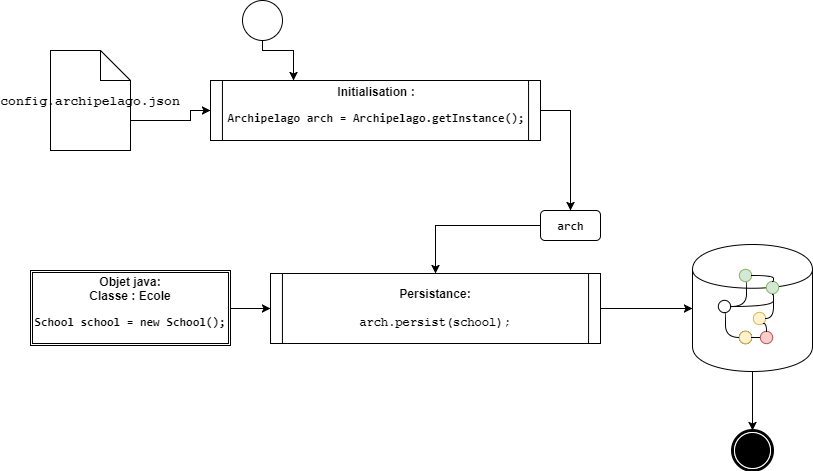
\includegraphics[scale=0.5]{figures/Persist.png}
\caption{Flux de persistance d'un objet au travers du framework Archipelago}
\label{fig:Persist}
\end{figure}
    
Pour ce qui est de la persistance du lien entre deux objets, nous avons fait le choix de créer des relations unidirectionnelles. Afin de créer un lien, il faut apposer l'annotation \textit{@Bridge} sur la propriété d'où il part.

Nous avons cependant ajouté la possibilité d'obtenir une relation réciproque en associant la valeur \texttt{true} dans l'attribut \texttt{biDirectionnal} de l'annotation. 

Exemple avec la Classe \textit{Student.java}

\begin{lstlisting}
public class Student extends Person {

    @Bridge(descriptor = "Follow")
    private List<Lesson> lessons = new ArrayList<>();
    
    @Bridge(descriptor = "FriendOf")
    private List<Student> friends = new ArrayList<>();
    
    @Bridge(descriptor = "FamilyMember", biDirectionnal = true)
    private List<? extends Person> familyMember = new ArrayList<>();
    
    @Bridge(descriptor = "PromotedIn")
    private Promotion prom;
    
    ...
    
\end{lstlisting}

Le \texttt{descriptor} qui est obligatoire, se doit d'être unique, il va représenter dans le BDOG le type de lien entre deux nœuds.

La beauté derrière cette utilisation est qu'au moindre changement de modèle, comme un ajout de propriété, l'ensemble de la couche de persistance sera adaptée à ce changement sans devoir exécuter le moindre script (à l'exception de la création d'une nouvelle classe pour OrientDB).

Si nous prenons l'exemple de l'école (méthode en annexe \ref{SchoolObj}) nous pouvons réaliser qu'en un seul graphe, nous visualisons l'ensemble des relations, qu'elles soient uni ou bidirectionnelles.

\begin{lstlisting}
Archipelago arch = Archipelago.getInstance();

School school = genSchool()

arch.persist(gilles);
\end{lstlisting}

\begin{figure}[!ht]
\centering
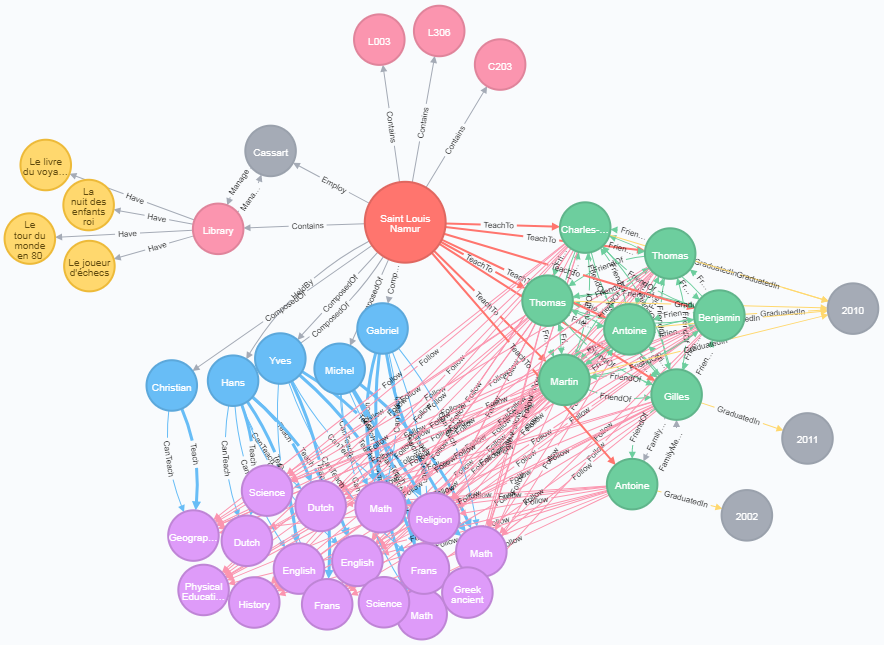
\includegraphics[scale=0.53]{figures/ecoleNeo4J.png}
\caption{Graphe généré dans Néo4J après appel de la méthode persist du framework Archipelago}
\label{fig:ecoleNeo4J}
\end{figure}

\subsection{La liaison}

Tout graphe se doit de pouvoir lier deux nœuds entre eux, Archipelago offre donc la possibilité de spécifier une liaison entre deux objets en utilisant un troisième. 

Voici un exemple : 

\begin{lstlisting}

Archipelago arch = Archipelago.getInstance();

City winterfell = new City("Winterfell");
City kingsLanding = new City("King's Landing");

Road road= new Road();
road.setDistance(500l);
road.setUnit("leagues");
        
arch.link(winterfell, kingsLanding, road);

\end{lstlisting}

Comme nous pouvons aisément le comprendre, nous allons lier ces deux villes par une relation "Road" contenant les propriétés "distance" et "unité".

\begin{figure}[!ht]
\centering
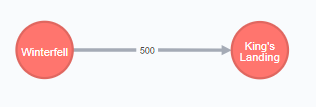
\includegraphics[scale=1.2]{figures/Rel.png}
\label{fig:Relation}
\caption{Résultat obtenu après utilisation de la méthode link d'Archipelago (avec Néo4J)}
\end{figure}

Toutefois si nous le spécifions à l'aide de la valeur "true" , le quatrième attribut de la méthode nous permet de générer automatiquement une relation réciproque ou bidirectionnelle. 

\begin{lstlisting}
...
arch.link(winterfell, kingsLanding, road, true);
...
\end{lstlisting}


\begin{figure}[!ht]
\centering
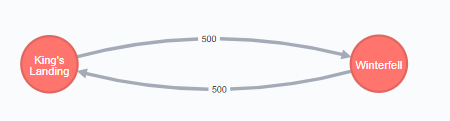
\includegraphics[scale=1.2]{figures/RelBidir.png}
\caption{Résultat obtenu après utilisation de la méthode link bidirectionnelle d'Archipelago (avec Néo4J)}
\label{fig:RelationBiDir}
\end{figure}

\subsection{La récupération}

La récupération de l'information est la raison pour laquelle nous la stockons. A quoi bon enregistrer une valeur dans une base de données si nous ne souhaitons jamais l'utiliser ultérieurement ?

Pour cela, Archipelago offre un système de création de requête. Grâce à ce procédé, que votre BDOG soit OrientDB ou Neo4J, vous serez en mesure de récupérer votre objet sans changer votre code source. 

Voici un exemple:

\begin{lstlisting}
Archipelago arch = Archipelago.getInstance();

ArchipelagoQuery aq = a.getQueryBuilder()
                .of(Student.class)
                .build();
List<Object> nodes = arch.execute(aq);
\end{lstlisting}

Cette requête va rechercher l'ensemble des étudiants de la base de données ainsi que les objets qui leur sont liés.

Un système de condition est également mis en place, il permet d'affiner le résultat obtenu: 

\begin{lstlisting}
Archipelago arch = Archipelago.getInstance();

ArchipelagoQuery aq = a.getQueryBuilder()
                .of(Student.class)
                .where(of("firstName","Gilles"), ConditionQualifier.Equal)
                .build();
List<Object> nodes = arch.execute(aq);
\end{lstlisting}

Cette requête va quant à elle rechercher les étudiants ayant "Gilles" comme prénom.

Nous pouvons aussi ajouter des opérateurs logiques "OU" et "ET" comme suit :
\begin{lstlisting}
Archipelago arch = Archipelago.getInstance();

ArchipelagoQuery aq = a.getQueryBuilder()
                .of(Student.class)
                .where(of("lastName", "Bodart"), ConditionQualifier.EQUAL)
                .and(of("firstName", "Gilles"), ConditionQualifier.EQUAL)
                .or(of("firstName", "Thomas"), ConditionQualifier.EQUAL)
                .build();
List<Object> nodes = arch.execute(aq);
\end{lstlisting}

Le procédé mis en place à l'heure actuelle ne permet pas de créer des conditions complexes car il va ajouter chaque élément de condition à la suite de la requête courante. 

Pour l'exemple précédent, nous aurons donc : 

\begin{lstlisting}[language=SQL]
(lastName = "Bodart" AND ( firstName = "Gilles" OR firstName = "Thomas"))
\end{lstlisting}

Comme expliqué plus haut, nous sommes actuellement dans l'incapacité de générer des requêtes comme suit :

\begin{lstlisting}[language=SQL]
(lastName = "Bodart" AND  firstName = "Gilles") 
 OR 
(lastName = "Blondiau" AND firstName = "Thomas")
\end{lstlisting}
\label{badCondition}
Dans notre troisième exemple, le système fournira donc la liste des étudiants ayant "Bodart" comme nom de famille et "Gilles" ou "Thomas" comme prénom. \`A L'heure actuelle, il n'est cependant pas possible d'effectuer des requêtes sur les relations entre les objets. Cette piste sera primordiale pour une deuxième version de ce framework.

\begin{figure}[!ht]
\centering
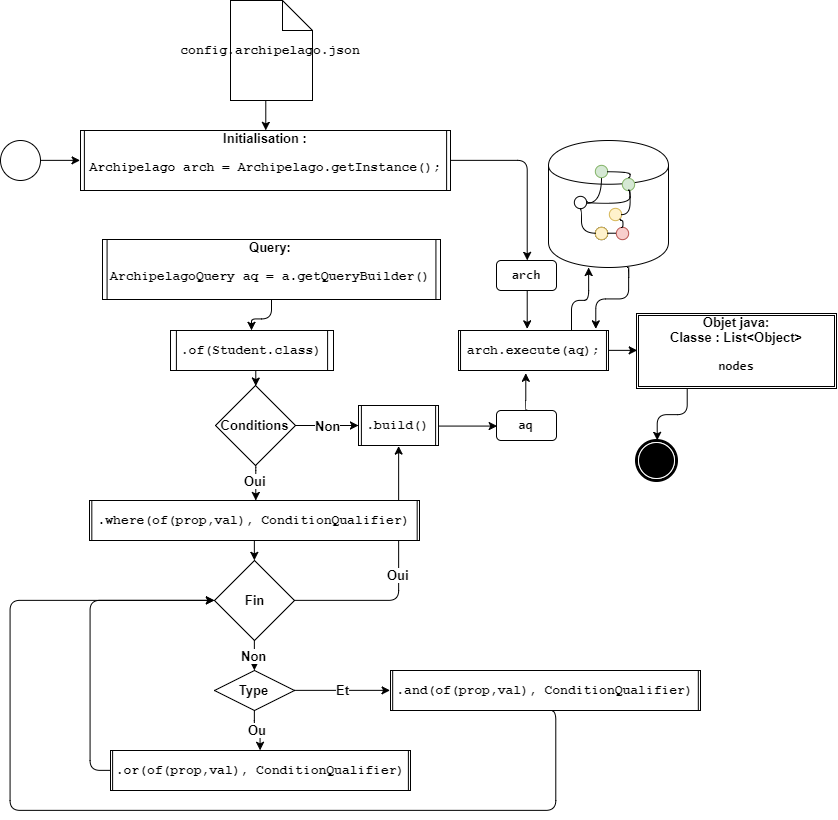
\includegraphics[scale=0.5]{figures/query.png}
\caption{Flux de traitement d'une requête de recherche dans Archipelago}
\label{fig:Query}
\end{figure}



\section{Schéma conceptuel}

La démarche suivie dans le cadre de ce travail est la suivante :

\begin{center}
\textbf{Abstraire la relation entre le code et la base de données, et accéder plus simplement à l’utilisation des BDOG. }
\end{center} 

Nous avons tenté de nous représenter le graphe dans l'univers de la programmation et nous nous sommes aperçu qu'il existait une grande divergence et une grande complexité entre les implémentations spécifiques des BDOG.

Nous nous sommes dès lors questionné sur la façon de s'éloigner de ces implémentations afin de ne plus être dépendants d'une représentation spécifique et de simplifier toute la procédure. Nous avons dès lors créé un ensemble d'éléments abstraits fournissant une interface entre des les différentes librairies préexistantes.

Archipelago est un framework qui permet d'utiliser ces librairies spécifiques des BDOG en reprenant sur base d’une configuration, les éléments nécessaires, et en simplifiant considérablement toutes les procédures de recherche et de création de requête.

Voici la démarche poursuivie :

\subsection{Archipelago}

L'objet principal du framework Archipelago est d'être une boite à outils comprenant les trois opérations décrites\footnote{voir \ref{opérations}} :
\begin{itemize}
\item La persistance
\item La liaison
\item La recherche
\end{itemize}

Grâce au fichier \texttt{config.archipelago.json}, l'environnement va se moduler automatiquement de manière à pouvoir exécuter le code spécifique adéquat.

Pour ces opérations, nous allons avoir besoin d'utilitaires nous permettant de générer des requêtes de persistance, de liaison et de recherche, pour chaque BDOG. Ces différentes implémentations doivent respecter les obligations décrites par les classes \texttt{ArchipelagoScriptBuilder} ainsi que \texttt{ArchipelagoQueryBuilder}.

Nous pensons que l'on pourrait fusionner ces deux classes. Néanmoins, nous avons opté pour le choix de les scinder afin de garder une différenciation entre les requêtes qui créent de l'information et celles qui en récupèrent.


\subsubsection{ScriptBuilders}


\begin{figure}[!ht]
\centering
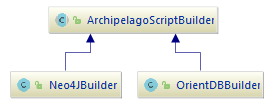
\includegraphics[scale=1.5]{figures/scriptBuilders.png}
\caption{Diagramme de classe représentant l'héritage des générateurs de script de persistance composant Archipelago}
\label{fig:ScriptQuery}
\end{figure}

Chaque classe doit correspondre à une base de données et implémenter trois méthodes\footnote{Plus un petit nombre d'overloading à implémenter} \footnote{Chacune de ces requêtes doit être écrite dans le langage ciblé par la classe.} :

\begin{tabular}[c]{|l|M{12cm}|}

\hline
\textbf{Nom de méthode} & \textbf{Description}  \tabularnewline
\hline
\texttt{makeCreate} &  Cette méthode doit générer une requête permettant de créer un nœud. \tabularnewline
\hline
\texttt{makeMatch} & Cette méthode doit générer une requête permettant de récupérer l'identifiant correspondant à un objet. \tabularnewline
\hline
\texttt{makeRelation} &  Cette méthode doit générer une requête permettant de lier deux nœuds.  \tabularnewline
\hline

\end{tabular}

\subsubsection{QueryBuilders}

\begin{figure}[!ht]
\centering
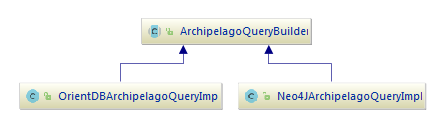
\includegraphics[scale=1.5]{figures/queryBuilders.png}
\label{fig:QueryBuilders}
\caption{Diagramme de classe représentant l'héritage des générateurs de script de recherche composant Archipelago}
\end{figure}

Comme précédemment, chaque classe doit correspondre à une base de données, la liste des méthodes à implémenter est légèrement plus importante.

En voici le détail :

\begin{tabular}[c]{|l|M{12cm}|}

\hline
\textbf{Nom de méthode} & \textbf{Description}  \tabularnewline
\hline
\texttt{init} & Initialisation de la requête de recherche.  \tabularnewline
\hline
\texttt{of} & Spécification de l'objet de la recherche.  \tabularnewline
\hline
\texttt{where} & Initialisation de conditions permettant de filtrer le résultat final.  \tabularnewline
\hline
\texttt{and} & Ajout d'une sous-condition liée avec un \texttt{ET} logique. \tabularnewline
\hline
\texttt{or} & Ajout d'une sous-condition liée avec un \texttt{OU} logique.   \tabularnewline
\hline
\texttt{build} & Finalise la requête de recherche de nœuds et génère une \texttt{ArchipelagoQuery}.   \tabularnewline \hline

\end{tabular}



\chapter{Evaluation}

Ce mémoire a été réalisé dans le but de développer un framework permettant d'abstraire les librairies spécifiques aux bases de données orientées graphe. Cependant, l'état actuel d'avancement de cet outil ne peut que le qualifier de "POC"\footnote{Proof of concept - Terme donné à un projet dont le but est de démontrer la faisabilité d'une approche d'architecture, d'une technologie ou d'une solution } \textcolor{blue}{todo livre}.


\section{Points forts}

\subsection{La facilité}

Grâce à Archipelago et sa méthode de persistance d'un objet java, il est aisé d'enregistrer des informations pouvant être fortement inter-connectées dans des bases de données orientées graphe. 
Le marquage des sommets lors de cette opération\textcolor{blue}{TODO livre} nous permet aussi d'améliorer les performances du procédé. 

\subsection{La configurabilité}

Nous avons choisi de prendre un fichier JSON comme fichier de configuration car ce format est simple d'utilisation. 

\`A l'heure actuelle, nous disposons d'un certain nombre de paramètres nous permettant d'orienter le framework vers l'une ou l'autre base de données et d'aider la récupération depuis ces dernières. De surcroît, le modèle mis en place permet aisément d'ajouter ou d'ôter de nouveaux paramètres en fonction des améliorations futures. 

\subsection{L'abstraction}

L'utilisateur ne doit se soucier d'aucune mise en œuvre spécifique à la base de données ciblée. 

Archipelago, grâce à ces  implémentations concrètes cachées derrière les classes abstraites \texttt{ArchipelagoScriptBuilder} ainsi que \texttt{ArchipelagoQueryBuilder} permet à l'exploiteur de se concentrer sur la partie algorithmique de son application.

\subsection{La simplification}

La manière dont nous avons imaginé ce framework permet de réutiliser n'importe quel code existant.Il suffit alors à l'utilisateur d'ajouter les annotations \texttt{@Bridge} pour que son code soit compatible avec l'application de ce framework. 

Il pourra ainsi profiter de bases de données NoSql orientées graphes, au lieu de s'en tenir aux bases de données relationnelles\footnote{voir \ref{noSqlVSRel}}; les frameworks de communication avec ces dernières étant plus courantes et mieux connues dans l'univers de la programmation.

\subsection{La modularité}

Chaque utilisation de librairie spécifique de communication vers une base de données extérieure se trouve dans une classe séparée.

Ce genre d'architecture offre une maintenance aisée car elle permet de concentrer la recherche de problèmes dans un espace défini et bien cadré. De plus, si deux équipes sont affectées simultanément à ce framework, elles peuvent y ajouter de nouvelles destinations sans se gêner, telles que par exemple ArangoDB\cite{arangoSite} ou encore JanusGraph\cite{janusGraphSite}. 


\section{Points faibles}
\subsection{Les performances}

Bien que nous ayons essayé d'améliorer ce point grâce au marquage des sommets, nous n'avons pas eu le temps d'approfondir ce procédé avec un marquage des arêtes. Dans notre exemple de l'école, la partie reprenant les étudiants est fortement inter-connectée. En conséquence nous devons passer à de nombreuses reprises sur les mêmes arêtes du graphe pour vérifier si cette relation existe dans la base de données au lieu de retenir l'information et d'éviter la démarche. Ces nombreux passages ralentissent le processus\footnote{Et plus particulièrement en ce qui concerne OrientDB}.

\subsection{Les conditions}

Notre framework possède trois faiblesses principales en ce qui concerne la manière avec laquelle nous pouvons récupérer de l'information.

\subsubsection*{\bf Sous-conditions}

Comme nous l'avons évoqué dans le point \ref{badCondition}, nous pouvons actuellement générer des conditions simples.
Pour créer des conditions plus complexes, il faudrait effectuer une refonte du système d'imbrication afin permettre à l'utilisateur de créer des sous-conditions. 

Exemple de condition impossible à générer actuellement :
\begin{lstlisting}[language=SQL]
(lastName = "Bodart" AND  firstName = "Gilles") 
 OR 
(lastName = "Blondiau" AND firstName = "Thomas")
\end{lstlisting}


\subsubsection*{\bf Conditions sur les relations}
De plus il n'est  pas possible de faire une condition sur une relation entre deux nœuds. 

Par exemple nous pourrions avoir grâce à la requête Cypher suivante : 

\begin{figure}[!ht]
\centering
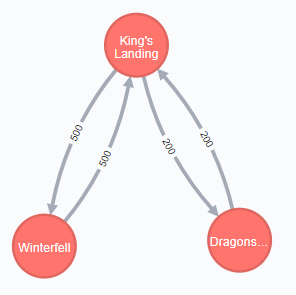
\includegraphics[scale=0.8]{figures/citiesRel.png}
\caption{Graphes Néo4J composé de 3 noeuds et de 4 relations}
\label{fig:citiesRel}
\end{figure}
 
\begin{lstlisting}[language=SQL]
MATCH (d:City)-[rel:Road]->(a:City)
WHERE
	    rel.distance > 300
	AND rel.unit = "leagues"
RETURN (a)
// Quelles sont les villes éloignées de plus de 300 lieues ?
\end{lstlisting} 


\begin{figure}[!ht]
\centering
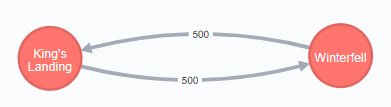
\includegraphics[scale=0.8]{figures/citiesRelFilt.png}
\label{fig:citiesRelFilt}
\caption{Graphes Néo4J composé de 2 noeuds et de 2 relations après exécution du filtre généré par Archipelago}
\end{figure}

Les requêtes générées par Archipelago nous permettent donc de récupérer l'ensemble des villes liées par une route, mais nous ne pourrons pas nous limiter à celles situées à plus de 300 lieues.

\subsubsection*{\bf Conditions sur les éléments liés}

Actuellement l'ensemble des conditions s'appliquent sur le nœud principal de la requête.

\`A cause de cela, il nous est impossible de filtrer les éléments qui vont être liés avec celui-ci. 

Voici un exemple en Cypher:

\begin{figure}[!ht]
\centering
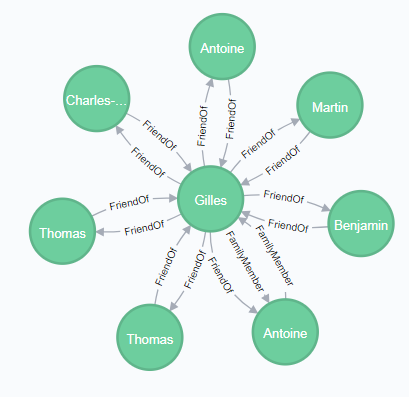
\includegraphics[scale=1]{figures/friendOf.png}
\label{fig:friendOf}
\caption{Graphe représentant les amis de "Gilles"}
\end{figure}
 
\begin{lstlisting}[language=SQL]
MATCH (me:Student)-[:FriendOf]->(f:Student)
WHERE
	    me.firstName = "Gilles"
	AND me.lastName = "Bodart"
	AND	f.firstName = "Thomas" 
RETURN (me)-[]-(f)
// lie-moi sont mes amis qui se prénomment Thomas?
\end{lstlisting} 

\begin{figure}[!ht]
\centering
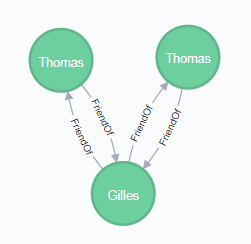
\includegraphics[scale=1]{figures/friendOfFilt.png}
\caption{Graphe représentant les amis de "Gilles" après exécution du filtre généré par Archipelago}
\label{fig:friendOfFilt}
\end{figure}

Archipelago à nouveau, ne permet pas de filtrer les amis liés au nœud principal. Du fait de ce manque de possibilité, nous sommes exposés à des problèmes de charge, dès lors que le nœud principal est lié à plusieurs millions d'autres.

\subsection{La récupération d'informations}

Dans l'état actuel d'avancement de ce framework, nous sommes en mesure d'enregistrer des informations sur les relations entre deux nœuds. Cependant il n'y a pas encore de procédé permettant de récupérer ces dernières dans un objet Java. Les  liaisons internes dans un objet seront récupérées mais nous ne bénéficierons pas de toutes les informations fournies lors de la persistance.

\begin{lstlisting}
public class City {

    private String name;

    @Bridge(descriptor = "Road")
    private List<City> connected = new ArrayList<>();
	
	...
\end{lstlisting}

\begin{lstlisting}
Archipelago arch = Archipelago.getInstance();
City winterfell = new City("Winterfell");
City kingsLanding = new City("King's Landing");
City dragonStone = new City("Dragonstone");

Road road= new Road();
road.setDistance(500l);
road.setUnit("leagues");

Road road2= new Road();
road2.setDistance(200l);
road2.setUnit("leagues");

a.persist(winterfell);
a.persist(kingsLanding);
a.persist(dragonStone);
a.link(kingsLanding,winterfell,road, true);
a.link(kingsLanding,dragonStone,road2, true);

ArchipelagoQuery aq = a.getQueryBuilder()
                .of(City.class)
                .where(of("name","King's Landing"), ConditionQualifier.EQUAL)
                .build();
                
List<Object> nodes = arch.execute(aq);
\end{lstlisting}

Nous récupèrerons le nœud correspondant à la ville "King's Landing" et nous aurons dans la propriété \texttt{connected} deux autres villes, à savoir "Dragonstone" et "Winterfell". Cependant, nous perdons dans l'application, les informations de distance et d'unité présentes dans les relations \texttt{Road}.


\subsection{La propreté du code}

Cette implémentation de ce framework pourrait être améliorée si l'on disposait de temps supplémentaire pour en évacuer les morceaux de codes inutiles. En outre, il serait primordial d'y insérer des tests unitaires afin de s'assurer du bon fonctionnement de chacune des méthodes implémentées.

Le code est actuellement disponible sur un "repository github"\footnote{https://github.com/GillesBodart/Archipelago}, de façon à pouvoir récupérer\footnote{Nous n'en avons pas encore reçu.} un ensemble de commentaires constructifs par la communauté Java. 

\chapter{Conclusion}


Archipelago est un framework dont le but est d'abstraire l'utilisation d'une BDOG orientée graphe. 

Le but de ce travail est de permettre à l'utilisateur de se centrer sur la représentation du modèle ainsi qu'au traitement métier de celui-ci, sans perdre du temps à implémenter la couche de persistance. L'état actuel du développement de ce framework peut être considéré comme un "POC".

Certaines fonctionnalités ont d'ores et déjà été implémentées telles que la persistance, la liaison et la récupération.

Comme signalé ci-dessus, nous pouvons reprendre les points forts de ce framework à savoir :

\begin{itemize}
\item \textbf{La facilité}

\quad La facilité d'enregistrement d'informations, pouvant être fortement inter-connectées dans des BDOG, ainsi que le marquage des sommets.

\item \textbf{La configurabilité}

\quad Une aide à la récupération d'un certain nombre de paramètres depuis un fichier de configuration permet de changer le comportement du framework ainsi que d'en ajouter ou d'en ôter aisément de nouveaux, en fonction des améliorations futures.

\item \textbf{L'abstraction}

\quad L'utilisateur ne doit se soucier d'aucune mise en œuvre spécifique à la base de données ciblée. 

\item \textbf{La simplification}

\quad Ce framework permet de réutiliser n'importe quel code existant. Il suffit alors à l'utilisateur d'ajouter les annotations \texttt{@Bridge} pour que son code soit compatible avec son application.

\item \textbf{La modularité}

\quad Le genre d'architecture utilisée pour développer ce framework, offre une maintenance aisée car elle permet de concentrer la recherche de problèmes dans un espace défini et bien cadré.

\end{itemize}

Les points faibles quant à eux sont :


\begin{itemize}
\item \textbf{Les performances}

\quad Bien que nous ayons essayé d'améliorer ce point grâce au marquage des sommets, nous n'avons pas eu le temps d'approfondir ce procédé avec un marquage des arêtes.

\item \textbf{Les conditions}

\quad Notre framework possède trois faiblesses principales en ce qui concerne la manière avec laquelle nous pouvons récupérer de l'information.
\begin{itemize}
	\item[•] \underline{Sous-conditions :} nous pouvons actuellement générer des conditions simples. Pour créer des conditions plus complexes, il faudrait effectuer une refonte du système d'imbrication afin permettre à l'utilisateur de créer des sous-conditions. 
	\item[•] \underline{Conditions sur les relations :} l'impossibilité de produire une condition sur une relation entre deux nœuds.
	\item[•] \underline{Conditions sur les éléments liés :} Actuellement l'ensemble des conditions s'appliquent sur le nœud principal de la requête , il nous est impossible de filtrer les éléments qui vont être liés avec celui-ci. Nous sommes dès lors exposés à des problèmes de charge si le nœud principal est lié à plusieurs millions d'autres.
\end{itemize}

\item \textbf{La récupération d'informations}

\quad Il n'existe pas encore de procédé permettant de récupérer des informations sur une relation entre deux nœuds, dans un objet Java. Les  liaisons internes dans un objet seront récupérées mais nous ne bénéficierons pas de toutes les informations fournies lors de la persistance.

\item \textbf{La propreté du code}

\quad L'implémentation de ce framework pourrait être améliorée si l'on disposait de temps supplémentaire pour en évacuer les morceaux de codes inutiles. En outre, il serait primordial d'y insérer des tests unitaires afin de s'assurer du bon fonctionnement de chacune des méthodes implémentées.

\end{itemize}  

L'ensemble de ces points faible à été pris en considération durant le développement de ce framework. Nous vous proposons dès lors des pistes d'améliorations réalistes telles que : 
\begin{enumerate}
\item Amélioration du système de conditions
\item Amélioration des performances
\item Amélioration de l'exploitation des relations
\item Ajout d'algorithmes célèbres de théorie des graphes
\end{enumerate}
 
Et nous les développerons dans le chapitre \ref{perspectives} de ce travail.

\vspace{1cm}

Si l'approche d'une mise en place d'un standard commun aux BDOG semblait intéressante en soi, elle irait apparemment à l'encontre même de ces systèmes. Même si Gremlin et OpenCypher sont en voie de s'imposer vu leur importance dans l'univers des BDOG, la plupart des leurs promoteurs souhaitent les considérer comme des bases de données spécialisées.

La solution proposée par ce mémoire permet quant à elle, d'abstraire les différentes implémentations standardisées ou non, et constituerait une approche unifiée pour l'univers des développeurs Java.

\chapter{Perspectives}
\label{perspectives}
\section{Amélioration du système de conditions}

Pour améliorer le système de conditions, il est primordial de refondre la manière dont les conditions sont implémentées. Pour l'avenir de ce projet, il faut que l'utilisateur soit en mesure d'émettre des conditions sur les relations ainsi que sur les éléments liés.

Sur base du questionnaire que nous avons soumis, une idée de modification est apparue dans les suggestions et nous a particulièrement convaincu. 

Le système pourrait être revu de la manière suivante : 

\begin{lstlisting}
Archipelago arch = Archipelago.getInstance();

ArchipelagoQuery aq = arch.getQueryBuilder()
    .of(City.class)
    .where(and(
              or(
      	          eq("name","King's Landing"),
    	          eq("name","Winterfell")
    	        ),
    	      neq("name","Dragonstone")
    	      ),
    	   ArchipelagoPosition.START
    	  )
    .where(and(
      	        gt("distance",300),
    	        eq("unit","leagues")
    	       ),
    	   ArchipelagoPosition.EDGE
    	  )
    .where(eq("name","Winterfell"),
    	   ArchipelagoPosition.END
    	  )
    .build();
List<Object> nodes = arch.execute(aq);

\end{lstlisting}

Avec ce procédé, chaque condition peut être imbriquée dans une autre sous-condition. Nous avons dès lors grâce à cette implémentation, la possibilité d'effectuer toutes les conditions logiques possibles sur le nœud de départ, sur l'arête ainsi que sur le nœud d'arrivée.

\section{Amélioration des performances}

Le premier effort, afin d'améliorer les performances, serait d'effectuer le marquage des arêtes.

Les algorithmes existant de la théorie des graphes, nous permettraient d'améliorer le parcours du graphe généré par les relations entre les différents objets du modèle.

\textcolor{blue}{théorie des graphes livre et algo}
\section{Amélioration de l'exploitation des relations}

Un objet générique représentant un lien entre deux objets peut être une piste d'amélioration de l'exploitation des relations. Comme la librairie de Néo4J le fait, la récupération d'information s'effectue entre autres dans un objet contenant 3 propriétés intéressantes :

\begin{tabular}[c]{l M{12cm}}
\texttt{start} & L'objet de départ.  \tabularnewline
\texttt{relation} & L'objet comprenant les informations de relation.  \tabularnewline
\texttt{end} & Le nœud d'arrivée.  \tabularnewline
\end{tabular}

Grâce à cette représentation, nous serons en mesure d'effectuer un grand nombre d'instructions sur ces relations essentielles dans l'utilisation d'une base de données orientée graphe.

\section{Ajout d'algorithmes célèbres de théorie des graphes}

\subsection*{Plus court chemin}

L'utilisation des BDOG est entre autres un choix pris pour effectuer des recherches de proximité entre deux éléments de la base de données. Ces algorithmes sont souvent déjà implémentés du côté des BDOG mêmes. Il faudrait dès lors qu'Archipelago implémente une nouvelle fonction permettant d'appeler ces algorithmes tels que le très célèbre "Dijkstra"\textcolor{blue}{livre sur dijkstra}. 

Exemple : 

\begin{lstlisting}
Archipelago arch = Archipelago.getInstance();

ArchipelagoQuery aq = arch.getQueryBuilder()
    .from(City.class)
    	.where(and(
              or(
      	          eq("name","King's Landing"),
    	          eq("name","Winterfell")
    	        ),
    	      neq("name","Dragonstone")
    	      ),
    	   ArchipelagoPosition.START
    	  )
    .to(City.class)
    	.where(eq("name","Winterfell"),
    	   ArchipelagoPosition.END
    	  )
    .with(ArchipelagoAlgo.DIJKSTRA)
    .build();
List<Object> nodes = arch.execute(aq);
\end{lstlisting}

\subsection*{Coloration des nœuds}

La coloration des nœuds est un procédé mathématique permettant de scinder un graphe en plusieurs groupes.
\textcolor{blue}{TODO à compléter}

\subsection*{Problème du voyageur de commerce}

Le problème du voyageur de commerce est un problème d'optimisation visant à lier un ensemble de nœuds en formant le plus court chemin entre ceux-ci.

Une implémentation d'une heuristique telle que par exemple l'ACS\cite{dorigo1997ant} peut être une fonctionnalité intéressante pour une seconde version de ce framework. En effet, si l'utilisateur à la possibilité d'employer ce genre d'algorithme pour résoudre ce type de problème, Archipelago répondra plus facilement aux attentes d'applications logistiques.



\textcolor{blue}{bd orienté réseaux}\cite{gardarin2003base}

\nocite{*}

\bibliography{biblio} 

\part{Annexes}
\section*{1. diagramme de classe "l'école"}

\begin{figure}[!ht]
	\centering
    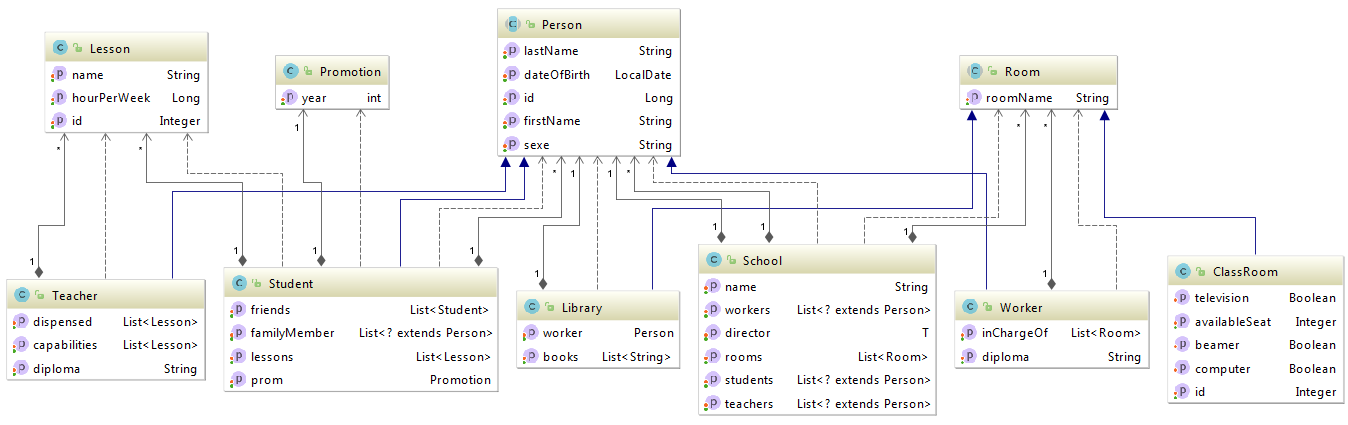
\includegraphics[angle=90,origin=c,scale=0.8]{figures/SchoolDiag.png}
    \caption{Diagramme de Classe du modèle École}
    \label{fig:SchoolDiagram}
\end{figure}

\section*{2. Création des objets composant l'école}

\begin{lstlisting}
private static School genSchool() throws ClassNotFoundException, IOException {

    Lesson math8 = new Lesson("Math", 8l);
    Lesson math6 = new Lesson("Math", 6l);
    Lesson math4 = new Lesson("Math", 4l);
    Lesson science6 = new Lesson("Science", 6l);
    Lesson science3 = new Lesson("Science", 3l);
    Lesson frans5 = new Lesson("Frans", 5l);
    Lesson frans6 = new Lesson("Frans", 6l);
    Lesson dutch2 = new Lesson("Dutch", 2l);
    Lesson dutch4 = new Lesson("Dutch", 4l);
    Lesson english2 = new Lesson("English", 2l);
    Lesson english4 = new Lesson("English", 4l);
    Lesson history = new Lesson("History", 2l);
    Lesson geography = new Lesson("Geography", 2l);
    Lesson religion = new Lesson("Religion", 2l);
    Lesson pE = new Lesson("Physical Education", 2l);
    Lesson greek = new Lesson("Greek ancient", 4l);
    Promotion p2011 = new Promotion(2011);
    Promotion p2002 = new Promotion(2002);
    Promotion p2010 = new Promotion(2010);
    Teacher gys = new Teacher("Hans", "Gys", null, "M", Lists.newArrayList(dutch2, dutch4, english2, english4), Lists.newArrayList(dutch2, dutch4,english2, english4), "Master");
    Teacher goffin = new Teacher("Michel", "Goffin", null, "M", Lists.newArrayList(math8, math6, math4), Lists.newArrayList(math8, math6, math4), "Master");
    Teacher massart = new Teacher("Gabriel", "Massart", null, "M", Lists.newArrayList(math8, math6, math4), Lists.newArrayList(math8, math6, math4), "Master");
    Teacher gouthers = new Teacher("Yves", "Gouthers", null, "M", Lists.newArrayList(frans5, frans6, religion), Lists.newArrayList(frans5, frans6, religion), "Master");
    Teacher jacques = new Teacher("Christian", "Jacques", null, "M", Lists.newArrayList(geography), Lists.newArrayList(geography), "Master");
    Student gilles = new Student("Gilles", "Bodart", LocalDate.of(1992, 4, 14), "M", Lists.newArrayList(math8, science6, dutch2, english4, history, geography, religion, frans5, pE), null, null, p2011);
    Student thomasB = new Student("Thomas", "Blondiau", LocalDate.of(1992, 1, 5), "M", Lists.newArrayList(math8, science3, dutch2, english4, history, geography, religion, frans5, pE, greek), null, null, p2010);
    Student thomasR = new Student("Thomas", "Reynders", LocalDate.of(1992, 1, 22), "M", Lists.newArrayList(math8, science6, dutch2, english4, history, geography, religion, frans5, pE), null, null, p2010);
    Student charly = new Student("Charles-Antoine", "Van Beers", LocalDate.of(1992, 4, 28), "M", Lists.newArrayList(math8, science3, dutch2, english4, history, geography, religion, frans5, pE, greek), null, null, p2010);
    Student antoine = new Student("Antoine", "Dumont", LocalDate.of(1992, 12, 28), "M", Lists.newArrayList(math6, science3, dutch4, english4, history, geography, religion, frans5, pE, greek), null, null, p2010);
    Student martin = new Student("Martin", "Périlleux", LocalDate.of(1992, 2, 28), "M", Lists.newArrayList(math6, science3, dutch4, english4, history, geography, religion, frans5, pE, greek), null, null, p2010);
    Student benjamin = new Student("Benjamin", "Leroy", LocalDate.of(1992, 10, 31), "M", Lists.newArrayList(math8, science3, dutch2, english4, history, geography, religion, frans5, pE, greek), null, null, p2010);
    Student antoineBo = new Student("Antoine", "Bodart", LocalDate.of(1985, 10, 18), "M", Lists.newArrayList(math6, science6, dutch2, english4, history, geography, religion, frans5, pE), null, null, p2002);
    Worker cassart = new Worker("", "Cassart", null, "M", null, null);
    List<Room> rooms;
    Room library = new org.archipelago.test.domain.school.Library("Library", Lists.newArrayList("Le livre du voyage", "Le tour du monde en 80 jours", "La nuit des enfants roi", "Le joueur d'échecs"), cassart);
    cassart.setInChargeOf(Lists.newArrayList(library));
    Room l003 = new ClassRoom("L003", 30, true, false, true);
    Room c203 = new ClassRoom("C203", 30, true, false, true);
    Room l306 = new ClassRoom("L306", 50, true, true, false);
    gilles.setFriends(Lists.newArrayList(thomasB, thomasR, charly, antoine, martin, benjamin, antoineBo));
    gilles.setFamilyMember(Lists.newArrayList(antoineBo));
    thomasB.setFriends(Lists.newArrayList(gilles, thomasR, charly, antoine, martin, benjamin));
    thomasR.setFriends(Lists.newArrayList(thomasB, gilles, charly, antoine, martin, benjamin));
    charly.setFriends(Lists.newArrayList(thomasB, thomasR, gilles, antoine, martin, benjamin));
    antoine.setFriends(Lists.newArrayList(thomasB, thomasR, charly, gilles, martin, benjamin));
    martin.setFriends(Lists.newArrayList(thomasB, thomasR, charly, antoine, gilles, benjamin));
    benjamin.setFriends(Lists.newArrayList(thomasB, thomasR, charly, antoine, martin, gilles));
    School school = new School();
    school.setName("Saint Louis Namur");
    school.setDirector(gys);
    school.setTeachers(Lists.newArrayList(goffin, gouthers, jacques, gys, massart));
    school.setStudents(Lists.newArrayList(gilles, thomasB, thomasR, charly, antoine, martin, benjamin, antoineBo));
    school.setRooms(Lists.newArrayList(library, l003, l306, c203));
    school.setWorkers(Lists.newArrayList(cassart));
    return school;
    }
\end{lstlisting}
\label{SchoolObj}

\chapter*{Code Sources}

%\textbf{Bridge.java}
\lstinputlisting{../Archipelago-core/src/main/java/org/archipelago/core/annotations/Bridge.java}
\textbf{ArchipelagoQuery.java}
\lstinputlisting{../Archipelago-core/src/main/java/org/archipelago/core/builder/ArchipelagoQuery.java}
\textbf{ArchipelagoScriptBuilder.java}
\lstinputlisting{../Archipelago-core/src/main/java/org/archipelago/core/builder/ArchipelagoScriptBuilder.java}
\textbf{ConditionQualifier.java}
\lstinputlisting{../Archipelago-core/src/main/java/org/archipelago/core/builder/ConditionQualifier.java}
\textbf{Neo4JBuilder.java}
\lstinputlisting{../Archipelago-core/src/main/java/org/archipelago/core/builder/Neo4JBuilder.java}
\textbf{Neo4JQueryImpl.java}
\lstinputlisting{../Archipelago-core/src/main/java/org/archipelago/core/builder/Neo4JQueryImpl.java}
\textbf{OrientDBBuilder.java}
\lstinputlisting{../Archipelago-core/src/main/java/org/archipelago/core/builder/OrientDBBuilder.java}
\textbf{OrientDBQueryImpl.java}
\lstinputlisting{../Archipelago-core/src/main/java/org/archipelago/core/builder/OrientDBQueryImpl.java}
\textbf{QueryBuilder.java}
\lstinputlisting{../Archipelago-core/src/main/java/org/archipelago/core/builder/QueryBuilder.java}
\textbf{QueryElement.java}
\lstinputlisting{../Archipelago-core/src/main/java/org/archipelago/core/builder/QueryElement.java}
\textbf{ArchipelagoConfig.java}
\lstinputlisting{../Archipelago-core/src/main/java/org/archipelago/core/configurator/ArchipelagoConfig.java}
\textbf{DatabaseConfig.java}
\lstinputlisting{../Archipelago-core/src/main/java/org/archipelago/core/configurator/DatabaseConfig.java}
\textbf{DatabaseType.java}
\lstinputlisting{../Archipelago-core/src/main/java/org/archipelago/core/configurator/DatabaseType.java}
\textbf{DescriptorWrapper.java}
\lstinputlisting{../Archipelago-core/src/main/java/org/archipelago/core/domain/DescriptorWrapper.java}
\textbf{OrientDBCluster.java}
\lstinputlisting{../Archipelago-core/src/main/java/org/archipelago/core/domain/OrientDBCluster.java}
\textbf{OrientDBErrorWrapper.java}
\lstinputlisting{../Archipelago-core/src/main/java/org/archipelago/core/domain/OrientDBErrorWrapper.java}
\textbf{OrientDBRelationWrapper.java}
\lstinputlisting{../Archipelago-core/src/main/java/org/archipelago/core/domain/OrientDBRelationWrapper.java}
\textbf{OrientDBResponseWrapper.java}
\lstinputlisting{../Archipelago-core/src/main/java/org/archipelago/core/domain/OrientDBResponseWrapper.java}
\textbf{OrientDBResultWrapper.java}
\lstinputlisting{../Archipelago-core/src/main/java/org/archipelago/core/domain/OrientDBResultWrapper.java}
\textbf{RelationWrapper.java}
\lstinputlisting{../Archipelago-core/src/main/java/org/archipelago/core/domain/RelationWrapper.java}
\textbf{CheckException.java}
\lstinputlisting{../Archipelago-core/src/main/java/org/archipelago/core/exception/CheckException.java}
\textbf{Archipelago.java}
\lstinputlisting{../Archipelago-core/src/main/java/org/archipelago/core/framework/Archipelago.java}
\textbf{ArchipelagoUtils.java}
\lstinputlisting{../Archipelago-core/src/main/java/org/archipelago/core/util/ArchipelagoUtils.java}
\textbf{StringTemplateFactory.java}
\lstinputlisting{../Archipelago-core/src/main/java/org/archipelago/core/util/StringTemplateFactory.java}


 

\end{document}
